\section{Modeling}
\label{sec:Modeling}

The structure of the considered building energy system is shown in Figure~\ref{fig:house_structure}.
Conventional heat generators such as boilers, CHP units, electrical heaters (EHs) and HPs are considered.
Furthermore, storage devices like electrical batteries (BATs) and TES units are available.
Solar generators like PV modules and STCs as well as peripheral devices like inverters are also included as possible parts of the optimal BES.
Thermal loads include space heating as well as domestic hot water.
Electrical loads describes the building's electricity consumption for lighting and electrical appliances.

\begin{figure}[h!]
	\begin{center}
		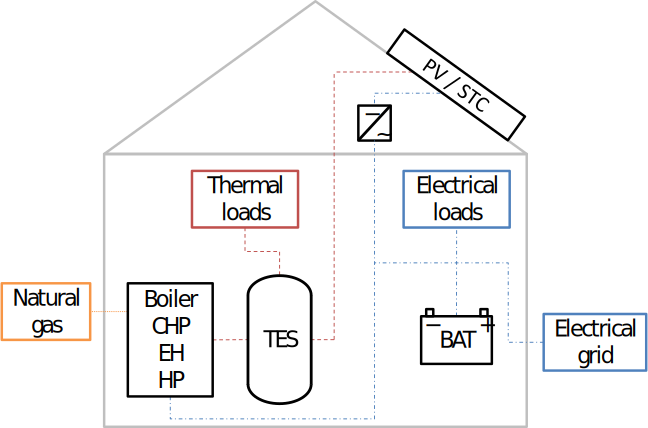
\includegraphics[width=\linewidth]{figures/house.pdf}
		\caption{Building energy system structure (single column figure)}
		\label{fig:house_structure}
	\end{center}
\end{figure}

The model requires annual inputs for these thermal and electrical loads.
Further inputs include device specific data, such as the available types (e.g. CHP unit 1, CHP unit 2, etc.) of each device (CHP, HP, etc.) and their characteristics, such as efficiency curves, expected life time, investment costs as well as operation and maintenance costs.
Also, information regarding different gas and electricity tariffs, economic parameters like interest rate, tax rates, length of the observation period and subsidy rates can be specified.

Since modeling an entire year requires long computing times, the framework also supports clustering the annual inputs into multiple representative periods that are weighted with weighting variables $\left(w_d\right)$.
The clustering is based on the k-medoids method \cite{Vinod1969,Dominguez-Munoz2011}, which has been shown to provide reliable results of high quality for energy system optimization purposes \cite{Schutz2016}.
If clustering is omitted, the weighting variables are set to 1.

The remainder of this section explains the objective functions as well as the economic, technical and ecological modeling.

\subsection{Objective functions}
The objectives of the developed model are minimization of annual costs $\left(c^\mathrm{ann}\right)$ and minimization of annual CO$_2$ emissions $\left(emi^\mathrm{ann}\right)$.
Annual costs are the sum of costs for investments $\left(c^\mathrm{inv}\right)$, operation and maintenance $\left(c^\mathrm{o\&m}\right)$, demand related costs $\left(c^\mathrm{dem}\right)$ and metering $\left(c^\mathrm{met}\right)$ less the revenues generated from feed-ins $\left(e^\mathrm{fin}\right)$ and governmental subsidies $\left(e^\mathrm{sub}\right)$.
\begin{equation}
	c^\mathrm{ann} = c^\mathrm{inv} + c^\mathrm{o\&m} + c^\mathrm{dem} + c^\mathrm{met} - e^\mathrm{fin} - e^\mathrm{sub}
	\label{eqn:obj_costs}
\end{equation}

Annual CO$_2$ emissions comprise emissions from gas usage $\left(emi^\mathrm{gas}\right)$, imported electricity $\left(emi^\mathrm{el,imp}\right)$ and negative emissions from electricity exports $\left(emi^\mathrm{el,exp}\right)$.
\begin{equation}
	emi^\mathrm{ann} = emi^\mathrm{gas} + emi^\mathrm{el,imp} - emi^\mathrm{el,exp}
\end{equation}

The following subsections describe the implemented constraints that limit the feasible search space.

\subsection{Economical constraints}
The economic modeling is based on the German engineering guideline VDI~2067 \cite{VDI_2067}, that has also been used in previous publications \cite{Harb2016,Schutz2016,Schutz2016a} \begin{LARGE}
\textbf{Applied Energy}
\end{LARGE}.

The following subsections define each element of the above mentioned parts of the economic objective.

\subsubsection{Investments}

According to this guideline, the investment costs are distributed into equal, annual payments by means of the capital recovery factor $\left(CRF\right)$.
The investment costs for each type $i$ of all devices $dev$, but PV and STC are computed as follows:
\begin{equation}
	c^\mathrm{inv}_{dev} = CRF \cdot tax^\mathrm{VAT} \cdot \sum\limits_{i} \left[ x_{dev,i} \cdot \left(1-rv_{dev,i}\right) \cdot c^\mathrm{inv}_{dev,i} \right]
\end{equation}

In this equation, $tax^\mathrm{VAT}$ represents the value added tax, $rv$ the residual value at the end of the period of interest, $c^\mathrm{inv}_{dev,i}$ the investment costs for each type of device and $x_{dev,i}$ the binary decision if type $i$ of device $dev$ is purchased or not.

For PV and STC the following equation is used, where $c^\mathrm{inv}_{dev,i}$ stands for module specific costs and $z_{dev,i}$ describes the number of installed modules of each type of collector.
\begin{equation}
	c^\mathrm{inv}_{dev} = CRF \cdot tax^\mathrm{VAT} \cdot \sum\limits_{i} \left[ z_{dev,i} \cdot \left(1-rv_{dev,i}\right) \cdot c^\mathrm{inv}_{dev,i} \right]
\end{equation}

The total investment costs mentioned in Eq.~\ref{eqn:obj_costs} are the sum of each devices' costs:
\begin{equation}
	c^\mathrm{inv} = \sum\limits_{dev} c^\mathrm{inv}_{dev}
	\label{eqn:sum_investments}
\end{equation}

The relationship shown in Eq.~\ref{eqn:sum_investments} is analogously applied to all subsequently described parts of the objective function and is therefore omitted in the following subsections.


\subsubsection{Operation and maintenance}

Costs for operation and maintenance are based on a fixed percentage $\left(f^{\mathrm{o\&m}}_{dev,i}\right)$ of the initial investment.
The corresponding values for $f^{\mathrm{o\&m}}_{dev,i}$ can be found in \cite{VDI_2067}.
For all devices but PV and STC, this relationship is modeled as:
\begin{equation}
	c^\mathrm{o\&m}_{dev} = b^{\mathrm{infl}} \cdot CRF \cdot tax^\mathrm{VAT} \cdot \sum\limits_{i} \left( x_{dev,i} \cdot c^\mathrm{inv}_{dev,i} \cdot f^{\mathrm{o\&m}}_{dev,i} \right)
	\label{eqn:costs_om_nonpvstc}
\end{equation}

In Eq.~\ref{eqn:costs_om_nonpvstc}, $b^{\mathrm{infl}}$ stands for the price dynamic cash value.
Analogously, this equation is formulated for PV and STC as follows:
\begin{equation}
	c^\mathrm{o\&m}_{dev} = b^{\mathrm{infl}} \cdot CRF \cdot tax^\mathrm{VAT} \cdot \sum\limits_{i} \left( z_{dev,i} \cdot c^\mathrm{inv}_{dev,i} \cdot f^{\mathrm{o\&m}}_{dev,i} \right)
\end{equation}

\subsubsection{Demand related costs}

Demand related costs depend on the chosen gas or electricity tariff.
If a CHP or boiler is installed, a gas tariff $\left(tar^\mathrm{gas}_{j}\right)$ has to be selected.
Furthermore, at most one gas tariff can be chosen.
\begin{align}
	\sum\limits_{j} tar^\mathrm{gas}_{j} &\ge \sum\limits_{i} x_{dev,i} \qquad \forall \; dev \in \left\lbrace\mathrm{CHP, BOI}\right\rbrace\\
	\sum\limits_{j} tar^\mathrm{gas}_{j} &\le 1
\end{align}

As many utilities offer a tiered pricing structure depending on the annual consumption, different tariff levels $\left(tar^\mathrm{gas,lvl}_{j,l}\right)$ are introduced.
At most one level can be valid and if the corresponding gas tariff is not chosen, all level variables have to be 0:
\begin{equation}
	\sum\limits_{l} tar^\mathrm{gas,lvl}_{j,l} = tar^\mathrm{gas}_{j}
\end{equation}

The correct level is bounded by a minimum annual consumption $\left(Gtar^\mathrm{LB}_{j,l}\right)$ and a maximum annual consumption $\left(Gtar^\mathrm{UB}_{j,l}\right)$:
\begin{equation}
	tar^\mathrm{gas,lvl}_{j,l} \cdot Gtar^\mathrm{LB}_{j,l} \le G^\mathrm{CHP}_{j,l} + G^\mathrm{BOI}_{j,l} \le tar^\mathrm{gas,lvl}_{j,l} \cdot Gtar^\mathrm{UB}_{j,l}
\end{equation}

In this equation, $G^\mathrm{CHP}_{j,l}$ and $G^\mathrm{BOI}_{j,l}$ describe the annual gas consumption of CHP units and boilers at tariff $j$ and level $l$.

For boilers and CHP units, the total gas consumption $G^\mathrm{tot}_{dev}$ of all days $d$ and time steps $t$ results in:
\begin{equation}
	G^\mathrm{tot}_{dev} = \sum\limits_{d} w_d \cdot \Delta t \cdot \sum\limits_{t} \sum\limits_{i} \dot{E}_{dev,i,d,t}
\end{equation}

In this equation, $\Delta t$ denotes the length of each time step, which has been set to one hour in this work.

The total gas consumption is distributed among the different levels of each tariff:
\begin{equation}
	G^\mathrm{tot}_{dev} = \sum\limits_{j} \sum\limits_{l} G^{dev}_{j,l}
\end{equation}

The demand related costs for gas consumption of boilers are computed with:
\begin{equation}
	c^{\mathrm{dem}}_{\mathrm{BOI}} = b^{\mathrm{gas}} \cdot CRF \cdot \sum\limits_{j} \sum\limits_{l} G^\mathrm{BOI}_{j,l} \cdot c^\mathrm{var,gas}_{j,l}
\end{equation}

For CHP units, a tax refund of $tax^{\mathrm{gas}}$ reduces the variable costs of $c^\mathrm{var,gas}_{j,l}$ \cite{EStG2015}:
\begin{equation}
	c^{\mathrm{dem}}_{\mathrm{CHP}} = b^{\mathrm{gas}} \cdot CRF \cdot \sum\limits_{j} \sum\limits_{l} G^\mathrm{CHP}_{j,l} \cdot \left( c^\mathrm{var,gas}_{j,l} - tax^{\mathrm{gas}} \right)
\end{equation}

Demand related electricity costs for purchases from the grid are modeled similarly to the costs for natural gas.
In contrast to the gas tariffs, at least one electricity tariff has to be chosen to satisfy plug loads:
\begin{equation}
	\sum\limits_{j^*} tar^{\mathrm{el}}_{j^*} = 1
	\label{eqn:el_tariffs plug loads}
\end{equation}

In Eq.~\ref{eqn:el_tariffs plug loads}, $j^*$ denotes all electricity tariffs that are not special heat pump tariffs.

If a heat pump is installed, a special heat pump tariff $hpt$ may be installed:
\begin{equation}
	tar^{\mathrm{el}}_{hpt} \le \sum\limits_{i} x_{i}^\mathrm{HP}
\end{equation}


Tiered pricing structures for electricity tariffs are modeled in a similar manner as for gas tariffs.
At most one level can be valid and if the corresponding electricity tariff is not chosen, all level variables have to be 0:
\begin{equation}
\sum\limits_{l} tar^\mathrm{el,lvl}_{j,l} = tar^\mathrm{el}_{j}
\end{equation}

The correct level is bounded by a minimum annual consumption $\left(Etar^\mathrm{LB}_{j,l}\right)$ and a maximum annual consumption $\left(Etar^\mathrm{UB}_{j,l}\right)$:
\begin{equation}
tar^\mathrm{el,lvl}_{j,l} \cdot Etar^\mathrm{LB}_{j,l} \le El^\mathrm{HOU}_{j,l} + El^\mathrm{HP}_{j,l} \le tar^\mathrm{el,lvl}_{j,l} \cdot Etar^\mathrm{UB}_{j,l}
\end{equation}

In this equation, $El^\mathrm{HOU}_{j,l}$ and $El^\mathrm{HP}_{j,l}$ describe the annual electricity purchases for the house's plug loads and HP at tariff $j$ and level $l$.
Since the HP tariff cannot be used to cover the house's plug loads, $El^\mathrm{HOU}_{hpt,l}$ is set to 0.

These total electricity imports are:
\begin{equation}
	El^\mathrm{tot}_{type} = \sum\limits_{d} w_d \cdot \Delta t \cdot \sum\limits_{t} \sum\limits_{i} P^{\mathrm{imp,}type}_{d,t} \qquad \forall \; type \in \left\lbrace\mathrm{HOU; HP}\right\rbrace
\end{equation}

The total amount of electricity imports is distributed among the different levels of each tariff:
\begin{equation}
	El^\mathrm{tot}_{type} = \sum\limits_{j} \sum\limits_{l} El^{type}_{j,l}
\end{equation}

Finally, the demand related costs are computed with:
\begin{equation}
c^{\mathrm{dem}}_\mathrm{el} = b^{\mathrm{el}} \cdot CRF \cdot \sum\limits_{type} \sum\limits_{j} \sum\limits_{l} El^{type}_{j,l} \cdot c^\mathrm{var,el}_{j,l}
\end{equation}

\subsubsection{Metering costs}

Metering costs directly follow from the chosen tariff and the resulting level. For gas tariffs the following equation is used:
\begin{equation}
	c^\mathrm{met}_{\mathrm{gas}} = \sum\limits_{j} \sum\limits_{l} tar^\mathrm{gas,lvl}_{j,l} \cdot c^\mathrm{fix,gas}_{j,l}
\end{equation}

In this equation, $c^\mathrm{fix,gas}_{j,l}$ denotes the fixed, annual metering costs of tariff $j$ and level $l$.
Fixed electricity metering costs are modeled analogously.

\subsubsection{Revenues from feed-in}

According to the German Renewable Energy Sources Act \cite{EEG2014}, electricity from PV is fed into the grid at a constant remuneration rate of $p^\mathrm{f-in,PV}=0.1231\,\mathrm{EUR}/\mathrm{kWh}$:
\begin{equation}
	e^\mathrm{f-in}_{\mathrm{PV}} = b^\mathrm{EEG} \cdot CRF \cdot p^\mathrm{f-in,PV} \cdot \Delta t \cdot \sum\limits_{d} \sum\limits_{t} P^{\mathrm{sell}}_{\mathrm{PV},d,t}
\end{equation}

Electricity surplus from CHP can be fed into the grid at standard market rates, which are approx. $p^\mathrm{f-in,CHP}=0.038\,\mathrm{EUR}/\mathrm{kWh}$:
\begin{equation}
	e^\mathrm{f-in}_{\mathrm{CHP}} = b^\mathrm{EEG} \cdot CRF \cdot p^\mathrm{f-in,CHP} \cdot \Delta t \cdot \sum\limits_{i} \sum\limits_{d} \sum\limits_{t} P^{\mathrm{sell}}_{\mathrm{CHP},i,d,t}
\end{equation}

\subsubsection{Subsidies}
\label{ssec:subsidies}

In this paper, we consider subsidies for CHP units according to \cite{KWKG2016} and subsidies for battery systems based on \cite{KfW275_2016}.

For large micro CHP units above 2~kW rated electrical power (subset $i^*$), the subsidies are computed as:
\begin{equation}
	e^\mathrm{sub}_{\mathrm{CHP,large}} = b^\mathrm{EEG} \cdot CRF \cdot \Delta t \cdot \sum\limits_{i^*} \sum\limits_{d} w_d \cdot \sum\limits_{t} \left[p^\mathrm{sub,CHP}_{\mathrm{self}} \cdot \left(P^\mathrm{HOU}_{\mathrm{CHP,}i^*,d,t} + P^\mathrm{HP}_{\mathrm{CHP,}i^*,d,t}\right) + p^\mathrm{sub,CHP}_{\mathrm{sell}} \cdot P^\mathrm{sell}_{\mathrm{CHP,}i^*,d,t}\right]
	\label{eqn:subs_CHP_large}
\end{equation}

In this equation, $p^\mathrm{sub,CHP}_{\mathrm{self}}=0.04\,\mathrm{EUR}/\mathrm{kWh}$ denotes the subsidies for self-consumed electricity from CHP units and $p^\mathrm{sub,CHP}_{\mathrm{sell}}=0.08\,\mathrm{EUR}/\mathrm{kWh}$ the subsidies for sold power \cite{KWKG2016}.

Smaller micro CHP units (subset $i_*$) can either receive a fixed or a variable subsidy.
The fixed subsidies are computed with:
\begin{equation}
	sub^\mathrm{fix} = CRF \cdot t^\mathrm{max} \cdot p^\mathrm{sub,CHP}_{\mathrm{fix}} \cdot \sum\limits_{i_*} x_{\mathrm{CHP,}i_*} \cdot P^\mathrm{nom}_{\mathrm{CHP,}i_*}
\end{equation}

Here, $t^\mathrm{max}$ stands for the subsidized time of 60000 hours and $p^\mathrm{sub,CHP}_{\mathrm{fix}}=0.04\,\mathrm{EUR}/\mathrm{kWh}$ is the specific subsidy.

Variable subsidies for small scale CHP units are computed just like for large scale CHPs as described in Eq.~\ref{eqn:subs_CHP_large}, however they are stored in variable $sub^\mathrm{var}$.
Since the maximum of both, $sub^\mathrm{fix}$ and $sub^\mathrm{var}$ will be used by investors, the following equations model $e^\mathrm{sub}_{\mathrm{CHP,small}} = \max\left\lbrace sub^\mathrm{fix}; sub^\mathrm{var} \right\rbrace$ in a linear manner \cite{Williams2013}.
\begin{align}
	e^\mathrm{sub}_{\mathrm{CHP,small}} &\ge sub^\mathrm{fix}\\
	e^\mathrm{sub}_{\mathrm{CHP,small}} &\ge sub^\mathrm{var}\\
	e^\mathrm{sub}_{\mathrm{CHP,small}} &\le sub^\mathrm{fix} + M^\mathrm{fix} \cdot \delta^\mathrm{var}\\
	e^\mathrm{sub}_{\mathrm{CHP,small}} &\le sub^\mathrm{var} + M^\mathrm{var} \cdot \left(1 - \delta^\mathrm{var} \right)
\end{align}

In this set of equations, $M^\mathrm{fix} = CRF \cdot t^\mathrm{max} \cdot p^\mathrm{sub,CHP}_{\mathrm{fix}} \cdot 2\,\mathrm{kW}$ is an upper bound for the fixed subsidies, $M^\mathrm{var} = b^\mathrm{EEG} \cdot CRF \cdot 8760\,\mathrm{h} \cdot p^\mathrm{sub,CHP}_{\mathrm{sell}} \cdot 2\,\mathrm{kW}$ for the variable subsidies and $\delta^\mathrm{var}$ denotes a binary variable that is 1 if the variable subsidy option is chosen.

The overall subsidies for CHP units result in:
\begin{equation}
	e^\mathrm{sub}_{\mathrm{CHP}} = e^\mathrm{sub}_{\mathrm{CHP,small}} + e^\mathrm{sub}_{\mathrm{CHP,large}}
\end{equation}

Batteries are subsidized by the German Reconstruction Credit Institute \cite{KfW275_2016}.
This subsidy is essentially a relatively cheap credit, however only 75\% of this credit have to be repaid.
Therefore, we consider 25\% of this credit as a subsidy for battery storages.
The subsidies are capped by the actual investments less $sub_{\mathrm{BAT}}=1600\,\mathrm{EUR}/\mathrm{kW}$ times the installed peak PV power, and a maximum specific amount of $sub^\mathrm{max}_\mathrm{BAT}=2000\,\mathrm{EUR}/\mathrm{kW}$:
\begin{align}
	e^\mathrm{sub}_{\mathrm{BAT}} &\le 0.25 \cdot CRF \cdot sub^\mathrm{max}_\mathrm{BAT} \cdot \zeta^\mathrm{sub}_{\mathrm{BAT}}\\
	e^\mathrm{sub}_{\mathrm{BAT}} &\le 0.25 \cdot \left(c^\mathrm{inv}_{\mathrm{PV}} + c^\mathrm{inv}_{\mathrm{BAT}} - CRF \cdot sub_{\mathrm{BAT}} \cdot \zeta^\mathrm{sub}_{\mathrm{BAT}} \right) 
\end{align}

In this set of equations, $\zeta^\mathrm{sub}_{\mathrm{BAT}}$ stands for the product of installed PV power and the decision if a battery storage is installed.
According to Williams \cite{Williams2013}, this product is linearized as follows:
\begin{align}
	\zeta^\mathrm{sub}_{\mathrm{BAT}} &\le \sum\limits_{i} P^\mathrm{nom}_{\mathrm{PV},i} \cdot z_{\mathrm{PV,}i}\\
	\zeta^\mathrm{sub}_{\mathrm{BAT}} &\le \max_j\left\lbrace P^\mathrm{nom}_{\mathrm{PV,}j} \cdot \dfrac{A^\mathrm{max}}{A_{\mathrm{PV,}j}} \right\rbrace \cdot \sum\limits_{i} x_{\mathrm{BAT,}i}\\
	\zeta^\mathrm{sub}_{\mathrm{BAT}} &\ge \sum\limits_{i} P^\mathrm{nom}_{\mathrm{PV},i} \cdot z_{\mathrm{PV,}i} - \left(1 - \sum\limits_{i} x_{\mathrm{BAT,}i}\right) \cdot \max_j\left\lbrace P^\mathrm{nom}_{\mathrm{PV,}j} \cdot \dfrac{A^\mathrm{max}}{A_{\mathrm{PV,}j}} \right\rbrace
\end{align}

\subsection{Technical constraints}

The technical constraints comprise the device selection and their operation.

\subsubsection{Device selection}

At most one unit of each device (CHP, HP, etc.) can be chosen:
\begin{equation}
	\sum\limits_{i} x_{dev,i} \le 1
\end{equation}

For PV and STC, multiple modules $\left(z_{dev,i}\right)$ of each type may be chosen, as long as the available roof-top area $\left(A^\mathrm{max}\right)$ is not exceeded.
\begin{align}
	z_{dev,i} &\le x_{dev,i} \cdot \dfrac{A^\mathrm{max}}{A_{dev,i}}\\
	\sum\limits_{dev}\sum\limits_{i} z_{dev,i} \cdot A_{dev,i} &\le A^\mathrm{max}
\end{align}

The nominal heat provided by CHP, EH, boiler and HP has to exceed the design heat load (DHL) to ensure thermal comfort during cold weather conditions:
\begin{equation}
	\sum\limits_{i} \left(x_{dev,i} \cdot \dot{Q}^\mathrm{nom}_{dev,i}\right) \ge \dot{Q}^\mathrm{DHL}
\end{equation}

\subsubsection{Device operation}

Heating devices, such as boiler, CHP units, HP units and electrical heaters, can only be switched on, if they have been purchased.
The activation is modeled with a binary variable $y_{dev,i,d,t}$ that equals 1 if type $i$ of device $dev$ is activated during time step $t$ of day $d$:
\begin{equation}
	y_{dev,i,d,t} \le x_{dev,i}
\end{equation}

We use information regarding electricity consumption or generation $\left(P^\mathrm{mds}_{dev,i,d,t,k}\right)$, fuel input $\left(\dot{E}^\mathrm{mds}_{dev,i,d,t,k}\right)$ and heat output $\left(\dot{Q}^\mathrm{mds}_{dev,i,d,t,k}\right)$ provided in manufacturer's data sheets (mds) for each device to model the part load behavior.
As air-water heat pumps' efficiencies depend on outer conditions, time indexes ($d,t$) are necessary.
Index $k$ describes the node points of the provided performance charts of each device, where $k=0$ stands for the minimum part load and $k=K$ for nominal operation.

The following set of equations describes a piecewise linearization of the performance charts:
\begin{align}
	\dot{Q}_{dev,i,d,t} &= \sum\limits_{k} w_{dev,i,d,t,k} \cdot \dot{Q}^\mathrm{mds}_{dev,i,d,t,k}\\
	\dot{E}_{dev,i,d,t} &= \sum\limits_{k} w_{dev,i,d,t,k} \cdot \dot{E}^\mathrm{mds}_{dev,i,d,t,k}\\
	P_{dev,i,d,t} &= \sum\limits_{k} w_{dev,i,d,t,k} \cdot P^\mathrm{mds}_{dev,i,d,t,k}\\
	y_{dev,i,d,t} &= \sum\limits_{k} w_{dev,i,d,t,k}
\end{align}

The weighting variables $w_{dev,i,d,t,k}$ are either continuous variables for devices with free modulation range or binary variables for discrete part load stages.
Furthermore, $w_{dev,i,d,t,k}$ form a so called Special Order Set 2 (SOS2) that implies that at most two neighboring entries within $w_{dev,i,d,t,k}$ can be greater than zero at each time step \cite{Williams2013}.
The solver used in our simulations supports SOS2, however the SOS2 relationship can easily be reformulated by introducing additional binary variables \cite{Williams2013}.

The heat output of STC is:
\begin{equation}
	\dot{Q}_{\mathrm{STC,}i,d,t} = \eta_{\mathrm{STC,}i,d,t} \cdot z_{\mathrm{STC,}i} \cdot A_{\mathrm{STC,}i} \cdot I_{d,t}
\end{equation}

Where $\eta_{\mathrm{STC,}i,d,t}$ describes the device's efficiency based on the optical efficiency as well as linear and quadratic thermal losses.
The solar irradiation onto the collector is $I_{d,t}$ and is computed according to \cite{Duffie2013,Perez1990}.

The electricity generation from PV is modeled similarly, considering the average efficiency of inverters $\left(\eta_{\mathrm{INV}}\right)$:
\begin{equation}
	P_{\mathrm{PV,}i,d,t} = \eta_{\mathrm{PV,}i,d,t} \cdot z_{\mathrm{PV,}i} \cdot A_{\mathrm{PV,}i} \cdot I_{d,t} \cdot \eta_{\mathrm{INV}}
\end{equation}

The power from PV, CHP and the power discharging the BAT is split into self-consumption for general plug loads (HOU), the HP and electricity fed into the grid (sell).
For BAT and PV, these parts can be combined for all types of modules and batteries:
\begin{equation}
	\sum\limits_{i} P_{dev,i,d,t} = P^\mathrm{HOU}_{dev,d,t} + P^\mathrm{HP}_{dev,d,t} + P^\mathrm{sell}_{dev,d,t}
\end{equation}

In case of CHP units, a strict distinction between each type of CHP has to be made due to the precise modeling of CHP subsidies:
\begin{equation}
P_{\mathrm{CHP,}i,d,t} = P^\mathrm{HOU}_{\mathrm{CHP,}i,d,t} + P^\mathrm{HP}_{\mathrm{CHP,}i,d,t} + P^\mathrm{sell}_{\mathrm{CHP,}i,d,t}
\end{equation}

According to the German Renewable Energy Sources Act \cite{EEG2014}, at most 70\% of the generated PV power may be fed into the public grid.
If a battery system is installed and the subsidies described in Section~\ref{ssec:subsidies} are chosen, this number is even reduced to 50\% \cite{KfW275_2016}.
\begin{equation}
	P^\mathrm{sell}_{\mathrm{PV,}d,t} \le \sum\limits_{i} P^\mathrm{nom}_{\mathrm{PV,}i} \left[ 0.7 \cdot \left(z_{\mathrm{PV,}i} - \zeta^{\mathrm{PV,BAT}}_i \right) + 0.5 \cdot \zeta^{\mathrm{PV,BAT}}_i \right]
	\label{eqn:limit feed in}
\end{equation}

In Eq.~\ref{eqn:limit feed in}, $\zeta^{\mathrm{PV,BAT}}_i$ stands for the product of $z_{\mathrm{PV,}i}$ and $\sum\limits_{j} x_{\mathrm{BAT,}j}$ that is linearized as follows:
\begin{align}
	\zeta^{\mathrm{PV,BAT}}_i &\le z_{\mathrm{PV,}i}\\
	\zeta^{\mathrm{PV,BAT}}_i &\le \dfrac{A^{\mathrm{max}}}{A_{\mathrm{PV,}i}} \cdot \sum\limits_{j} x_{\mathrm{BAT,}j}\\
	\zeta^{\mathrm{PV,BAT}}_i &\ge z_{\mathrm{PV,}i} - \left(1- \sum\limits_{j} x_{\mathrm{BAT,}j}\right) \cdot \dfrac{A^{\mathrm{max}}}{A_{\mathrm{PV,}i}}
\end{align}

The inverter is sized according to the installed, nominal PV power:
\begin{equation}
	\sum\limits_{i} z_{\mathrm{PV,}i} \cdot P^\mathrm{nom}_{\mathrm{PV,}i} \le \sum\limits_{j} x_{\mathrm{INV,}j} \cdot P^\mathrm{nom}_{\mathrm{INV,}j}
\end{equation}

Storage units' energy contents are modeled based on their state of charge $S_{dev,i,d,t}$.
The state of charge can only be positive, if the corresponding device has been purchased:
\begin{equation}
	S_{dev,i,d,t} \le x_{dev,i}
\end{equation}

In order to allow a discrete selection of storage units, an energy balance is modeled for each type:
\begin{equation}
	S_{dev,i,d,t} = \left(1-\varphi_{dev,i}\right) \cdot S_{dev,i,d,t-1} + \Delta t \cdot \dfrac{\eta_{dev_i} \cdot ch_{dev,i,d,t} - dch_{dev,i,d,t}}{cap_{dev,i}}
	\label{eqn:soc_storages}
\end{equation}

The storage's relative standby losses between two consecutive time steps are $\varphi_{dev,i}$, $\eta_{dev_i}$ describes the storage cycle's efficiency, $ch_{dev,i,d,t}$ and $dch_{dev,i,d,t}$ stand for the charging and discharging energy and $cap_{dev,i}$ for the storage's capacity.
The capacity can be directly derived from data sheets for BATs.
For TES units, we calculate $cap_{dev,i}=\rho \cdot \kappa\cdot V_i \cdot \Delta T^\mathrm{max}$, where $\rho$ and $\kappa$ are the density and specific heat capacity of water, $V_i$ is the storage's volume and $\Delta T^\mathrm{max}=40\,\mathrm{K}$ the maximum temperature spread inside the tank.
Charging and discharging energy are restricted with big-M formulations, preventing the charging and discharging of tanks that have not been installed.
Appropriate bounds for BATs can be derived from data sheets and multiples of the design heat load are used for TES units.

For TES units, the following balances are applied to determine the charging and discharging energies:
\begin{align}
	\sum\limits_{i} ch_{\mathrm{TES,}i,d,t} &= \sum\limits_{dev^*} \sum\limits_{j} \dot{Q}_{dev^*,j,d,t}\\
	\sum\limits_{i} dch_{\mathrm{TES,}i,d,t} &= \dot{Q}^\mathrm{DHW}_{d,t} + \dot{Q}^\mathrm{SH}_{d,t}
\end{align}

In these formulations, $dev^*$ describes the subsets of all heat generating devices, $\dot{Q}^\mathrm{DHW}_{d,t}$ and $\dot{Q}^\mathrm{SH}_{d,t}$ describe the building's domestic how water and space heating demands at time $t$ on day $d$.
Both equations, in combination with the big-M constraints, ensure that all generated and demanded heat are interchanged with exactly one storage tank, nullifying all but one of the relationships presented in Eq.~\ref{eqn:soc_storages}

For BAT systems, the charging and discharging powers follow from the building's electricity balances.
We formulate one balance for the building's plug loads and a second balance for the electricity potentially billed with a special heat pump tariff.
The building's electricity balance is written as:
\begin{equation}
	P^\mathrm{HOU}_{d,t} + P^\mathrm{HOU}_{\mathrm{EH,}d,t} + \sum\limits_{i} ch_{\mathrm{BAT,}i,d,t} = P^\mathrm{imp,HOU}_{d,t} + P^\mathrm{HOU}_{\mathrm{PV,}d,t} + P^\mathrm{HOU}_{\mathrm{BAT,}d,t} + \sum\limits_{i} P^\mathrm{HOU}_{\mathrm{CHP,}i,d,t}
\end{equation}

Here, $P^\mathrm{HOU}_{d,t}$ describes the house's plug loads and $P^\mathrm{HOU}_{\mathrm{EH,}d,t}$ the amount of electricity provided by an EH that is not billed under a special heat pump tariff.

The second electricity balance is:
\begin{equation}
	\sum\limits_{i} P_{\mathrm{HP,}i,d,t} + P^\mathrm{HP}_{\mathrm{EH,}d,t} = P^\mathrm{imp,HP}_{d,t} + P^\mathrm{HP}_{\mathrm{PV,}d,t} + P^\mathrm{HP}_{\mathrm{BAT,}d,t} + \sum\limits_{i} P^\mathrm{HP}_{\mathrm{CHP,}i,d,t}
\end{equation}

The EHs electricity amounts are further described:
In total, the amount of electricity purchased at a potential heat pump tariff and the amount purchased at the standard tariff, have to be equal to the electricity consumption caused by this device:
\begin{equation}
	\sum\limits_{i} P_{\mathrm{EH,}i,d,t} = P^\mathrm{HOU}_{\mathrm{EH,}d,t} + P^\mathrm{HP}_{\mathrm{EH,}d,t}
\end{equation}

If no heat pump has been purchased, the electrical heater cannot be active in the second electricity balance:
\begin{equation}
	P^\mathrm{HP}_{\mathrm{EH,}d,t} \le \max_j\left\lbrace P^\mathrm{nom}_{\mathrm{EH},j} \right\rbrace \cdot \sum\limits_{i}x_{\mathrm{HP,}i}
\end{equation}

Finally, we prevent the heat pump from being activated if the storage temperature is above the heat pump's maximum flow temperature:
\begin{equation}
	\sum\limits_{i} S_{\mathrm{TES,}i,d,t} \le 1 - y_{\mathrm{HP,}j,d,t} \cdot \left( 1 - \dfrac{\Delta T^\mathrm{HP}}{\Delta T^\mathrm{max}} \right)
\end{equation}


\subsection{Ecological constraints}
We consider emissions from gas consumption and electricity purchase from the distribution grid as well as negative emissions for exporting electricity to the grid.

Considering the specific CO$_2$ emissions $\left(emi^\mathrm{gas,spec}_{j}\right)$ for each tariff $j$, the emissions from natural gas result in:
\begin{equation}
	emi^\mathrm{gas} = \sum\limits_{j} emi^\mathrm{gas,spec}_{j} \cdot \sum\limits_{l}  \left(G^\mathrm{CHP}_{j,l} + G^\mathrm{BOI}_{j,l}\right)
\end{equation}

Similarly, CO$_2$ emissions from electricity imports are modeled:
\begin{equation}
	emi^\mathrm{el,imp} = \sum\limits_{j} emi^\mathrm{el,spec}_{j} \cdot \sum\limits_{l} \left(El^\mathrm{HOU}_{j,l} + El^\mathrm{HP}_{j,l}\right)
\end{equation}

For computing negative emissions from electricity exports, we first compute the entire amount of exported electricity, $El^\mathrm{EXP,tot}$:
\begin{equation}
	El^\mathrm{EXP,tot} = \sum\limits_{d} w_d \cdot \Delta t \cdot \sum\limits_{t} \left[ \left( \sum\limits_{i} P_{\mathrm{CHP,}i,d,t}^\mathrm{sell} \right) + P_{\mathrm{PV},d,t}^\mathrm{sell} + P_{\mathrm{BAT,}d,t}^\mathrm{sell} \right]
\end{equation}

The following two equations ensure that electricity exports are attributed with the same CO$_2$ emissions as would occur for imports under the chosen tariff.
Since a special heat pump tariff could be selected in addition to a regular tariff, the subset $j^*$ denotes regular tariffs only.
\begin{equation}
	El^\mathrm{EXP,tot} = \sum\limits_{j^*} El^\mathrm{EXP}_{j^*}
\end{equation}
\begin{equation}
	El^\mathrm{EXP}_{j^*} \le tar_{j^*}^\mathrm{el} \cdot \max_l \left\lbrace Etar^\mathrm{UB}_{j^*,l} \right\rbrace
\end{equation}

Finally, the negative CO$_2$ emissions from electricity exports result in
\begin{equation}
	emi^\mathrm{el,exp} = \sum\limits_{j^*} emi^\mathrm{el,spec}_{j^*} \cdot El^\mathrm{EXP}_{j^*}
\end{equation}